\section{Evaluation}

In diesem Kapitel wird untersucht, ob und wie der umgesetzte Prototyp den Anforderungen an das System gerecht wird. Grundlage der Untersuchung ist das Testen des Prototypen. Ähnlich wie die Anforderungsanalyse, erfolgt auch die Evaluation für die Abstraktionsebenen Kontextebene, Systemebene und technologische Ebene. Auf Basis dieser Evaluationen wird schließlich eine passende Handlungsempfehlung für den Anwendungsfall gegeben. 

% Kontextebene
\subsection{Evaluation auf Kontextebene}
In der Kontextebene wurden Anforderungen an das System gestellt, welche sich aus den Einflussfaktoren im Systemkontext ergeben. Besonders die Probleme im Zusammenhang mit der Branche der Energiewirtschaft bilden die Kernanforderungen an das System (s. Anhang \ref{anfkontext}). Die sich daraus ergebenden funktionalen Anforderungen (K-FA-1) können im Großen und Ganzen als erfüllt betrachtet werden. Angefordert war es, dem Nutzer die Einsicht auf den digitalen Zwilling einer Anlage zu gewähren, einschließlich der Anzeige von Messwerten, Standorten und prädiktiven Informationen. Mit Betrachtung der Abbildungen \ref{thingpage}, \ref{landing}, \ref{detailoverview} und \ref{thingdetail} scheinen die Anforderungen erfüllt: Die Anlage wird auf der Startseite auf einer Landkarte verortet, die Übersicht über den Zustand liefert Bewertungen des Zustands und die Detailansicht listet einzelne Messwerte auf. Anhand der Einbindung des \ac{sns} von \ac{aws}, aber auch des Befehls zum Aufleuchten der LED, kann dem Wartungspersonal die Reaktion auf kritische Zustände ermöglicht werden. Probleme entstehen bei der Betrachtung der Anforderung \textit{Echtzeit}. Wie in Abbildung \ref{datavisual} dargestellt, werden die Daten sofort an die Cloud transferiert. Allerdings benötigt die Reaktion auf die Daten, also die Aktivierung der HTTP-Anfragen durch die Aktionen, eine Zeitspanne zwischen 20 Sekunden und 2 Minuten. Diese Zeitspanne ist zwar immer noch kürzer als der 10"=Minuten"=Takt des \ac{scada}-Systems, erfüllt aber nicht die Anforderung \textit{Echtzeit}. Nichtsdestotrotz werden die definierten Anwendungsfälle durch den Prototypen realisiert. 
Auch die qualitativen Anforderungen können größtenteils als erfüllt betrachtet werden. Die \ac{soa} von SAP Leonardo und der SAP Cloud Platform liefert die Flexibilität, das System an Veränderungen anzupassen, neue Funktionen einzubinden und neue Geräte hinzuzufügen. In diesem Prototypen wurde dies anhand von Destinationen realisiert. Zudem können über Schnittstellen weitere intelligente Dienste von SAP Leonardo und andere Funktionen (s. Abbildung \ref{leoae}) angebunden werden. Dass die Randbedingungen (K-RA-2 und K-RA-3) zur Orientierung an der \ac{rami} erfüllt werden, wird nach der Systemanalyse deutlich. Die Architektur von SAP Leonardo wird auf die Schichten der IT-Sicht von \ac{rami} angewandt. Das Ergebnis wird in Abbildung \ref{ramicustom} dargestellt. Allerdings wird in der Umsetzung der Kommunikation im Prototypen nicht, wie empfohlen, der OPC-UA-Standard verwendet. In der Systemanalyse wurde lediglich erwähnt, dass die Nutzung der OPC-UA über die Iot Edge Platform möglich ist.

% Systemebene
\subsection{Evaluation auf Systemebene}

Wie das System die Anforderungen aus der Kontextebene erfüllen soll, wurde in der Systemebene definiert. Der innerere logische Aufbau des umgesetzten Prototypen erfüllt mit einigen Schwachstellen die Anforderungen aus Anhang \ref{anf_system}.
Das Messinstrument sollte alle 5 Sekunden Daten erfassen und gemäß den Eigenschaften einer Industrie-4.0-Komponente an ein übergeordetes IT-System senden (S-FA-1). Mit Betrachtung der Abbildung \ref{datavisual} wird die Erfüllung dieser Anforderungen bestätigt. Auch die Virtualisierung der Anlage (S-FA-2) in einem digitalen Zwilling einschließlich der Funktionalisierung der eingehenden Daten wurde in der Implementierung erfolgreich umgesetzt. 
Schwachstellen zeigen sich eher aus qualitativer Sicht als aus funktionaler Sicht. Beim Testen des Prototypen unter Erhöhung der Temperatur über den angegebenen Grenzwert, wurde eine Unzuverlässigkeit des Systems beobachtet. Während bei einigen Versuchen die Aktionen wie das Senden der SMS und das Aufleuchten der LED sofort aktiviert wurden, gab es neben Versuchen mit Verzögerungen auch einige Fehlschläge. Der Empfang der SMS wird in Abbildung \ref{awsnoti} bestätigt. Die Ursache der Schwachstellen konnte allerdings nicht identifiziert werden. Es werden lediglich Verzögerungen im \textit{Message Processing} vermutet. Dies zeigt sich auch darin, dass die im Internet of Things Service zuverlässig empfangenen Messwerte sich nicht sofort in dem digitalen Zwilling der IoT-Anwendung aufzeigen. Ausgenommen von diesen Einzelheiten ist die Qualität des Systems gewährleistet. Ein Kriterium bezüglich der Eigenschaften einer Industrie-4.0-Komponente ist die Kommunikation in einem einheitlichen semantischen Datenformat. Sichergestellt wurde die einheitliche Kommunikation mit der Nutzung des \ac{json}-Datenformats in jeglichen APIs. Zudem wurde die Kommunikation über das Gateway durch das Einfügen von \textit{private Keys} für den Tenant der IoT Services gesichert. 



\begin{figure}[ht]
    \centering
    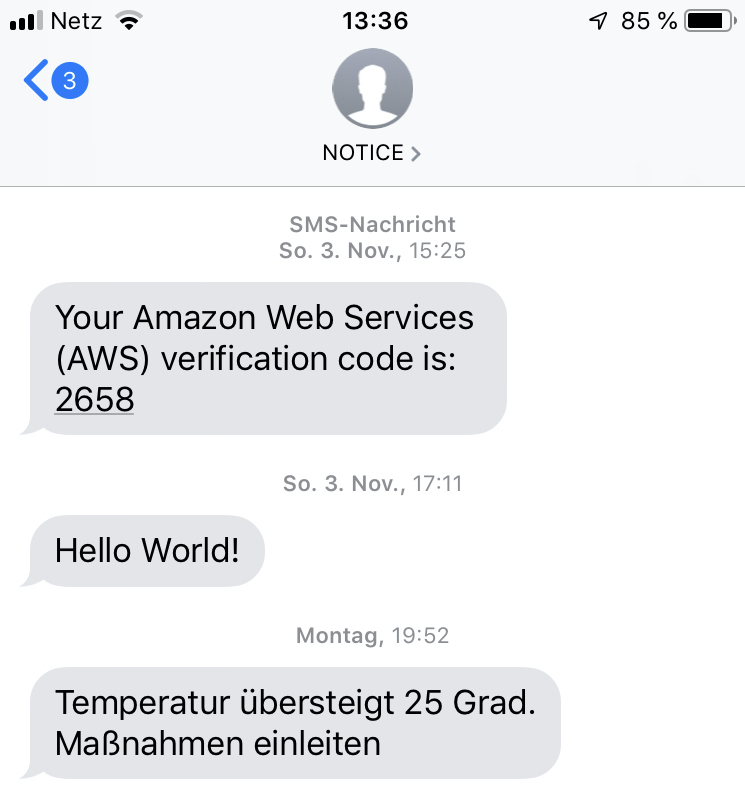
\includegraphics[width=0.6\linewidth]{AWS1_Notification.png}
    \caption{Empfang der Benachrichtigungs-SMS}
    \label{awsnoti}
\end{figure}

% technologische Ebene
\subsection{Evaluation auf technologischer Ebene}
Schwachstellen zeigen sich hinsichtlich der Visualisierung in einer Benutzerschnittstelle auf.  
Dass Echtzeit nicht immer erfüllt wird, deuetet auf Unzuverlässigkeit hin.
Message Processing lahm: Übertragung der Daten an digitalen Zwilling
\subsection{Handlungsempfehlung}
Anbindung der realen Anlagen über das OPC-UA Protokoll mit der Gateway Edge
Anbindung an HANA Datenbank, da schnellere In-Memrory Verarbeitung als PostGreSQL
Forschungsfragen
Anforderungen
Warten bis der Scheiß ausgereift ist aber auf jeden Fall an RAMI orientieren


Komplett Anforderungsanalyse abgleichen
Unflexible UI-Entwicklung weil Module und Packages nicht dokumentiert
OPC UA in Edge Möglich aber im Prototypen nicht implementiert

Abbildung \ref{datavisual} kann entnommen werden, dass die Daten zuverlässlig im 5-Sekunden-Takt empfangen werden. Problematisch ist die Verarbeitung in der Leo-Umgebung.
API Reaktionszeit schlecht und fehleranfällig und unzuverlässige Datenverarbeitung im SAP Leonardo IoT Regelwerk,
Regeln werden manchmal einfach nicht ausgelöst.


Das System bietet sicherlich mehr Möglichkeiten und ist bestimmt stabiler. Trotz umfassender API-Dokumentation ist der Nutzer des Systems nicht ausreichend mit Anwenderdokumentaion versorgt. Hilfreich sind die Blog-Beiträge der SAP-Community, welche jedoch nur anwendunfsfallbasierte Informationen liefern.
\newpage
